\chapter{Encoder Based Odometry for State Estimate}

\section{Overview}

In the platform previously described in chapter \ref{cha:Platform}, we have seen that two of it's wheel have encoders attached. These encoders give us a good estimate of the robot's movement in each time step. The function used to calculate the robot's movement from the encoder data is the motion model of the robot and is used for equation \ref{eq:EKF_1} in section \ref{sec:EKF}. Since this robot has only 3 degrees of freedom, our state vector, $ x \in \Re^3 $ and is defined as $ x = [x,y,\theta]^T $ where $ x $ and $ y $ give the position of the robot from an arbitrary fixed point in inertial frame of reference. 

\section{Motion model and the corresponding differentials}

To estimate the motion model, we first convert left and right wheel movement into distances traveled by them through a linear mapping using the known radius of the wheels. These values are represented by $ u = [ l, r ]^T $. The equations are better implemented as a piecewise function. We separately consider the cases when the robot is estimated to be going straight or to be turning. We can know this by just looking at the left and right distances. If they are exactly the same, the robot is going straight and the motion model is given by equations \ref{eq:Enc_1}. 

If $ r = l $:
\begin{equation}
\label{eq:Enc_1}
	\begin{bmatrix}
		\hat{x}^-\\\hat{y}^-\\\hat{\theta}^-
	\end{bmatrix}_k
	=
	\begin{bmatrix}
		\hat{x}\\\hat{y}\\\hat{\theta}
	\end{bmatrix}_{k-1}
	+
	\begin{bmatrix}
		l.\cos(\hat{\theta}_{k-1})\\
		l.\sin(\hat{\theta}_{k-1})\\
		0
	\end{bmatrix}
\end{equation}	

If not, we use equations \ref{eq:Enc_2} and \ref{eq:Enc_3}. Where $ R,\alpha $ and $ w $ are as shown in figure \ref{fig:Enc_1}
			
\begin{figure}
\centering
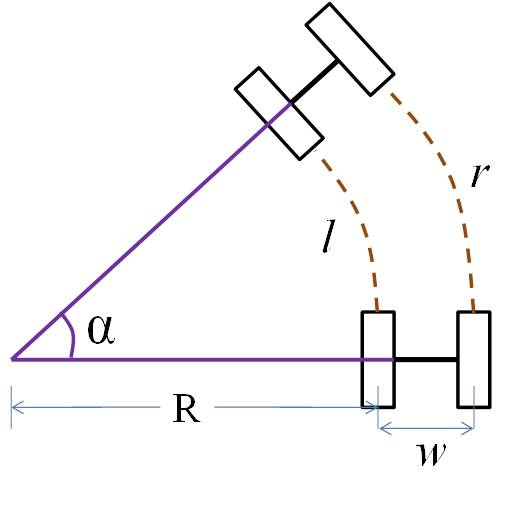
\includegraphics[width=0.3\textwidth,height=0.3\textheight]{differential_turning}
\caption{Motion model of Differential drive platform}
\label{fig:Enc_1}
\end{figure}
If $ r \neq l $:
\begin{equation}
\label{eq:Enc_2}
	\alpha= \frac{r-l}{w}
\qquad
	R=\frac{l}{\alpha}
\end{equation}
\begin{equation}
\label{eq:Enc_3}
	\begin{bmatrix}
		\hat{x}^-\\\hat{y}^-\\\hat{\theta}^-
	\end{bmatrix}_k
	=
	\begin{bmatrix}
		\hat{x}\\\hat{y}\\\hat{\theta}
	\end{bmatrix}_{k-1}
	+
	\begin{bmatrix}
		\left(R+\frac{w}{2}\right)(\sin(\hat{\theta}_{k-1}+\alpha)-\sin(\hat{\theta}_{k-1}))\\
		\left(R+\frac{w}{2}\right)(-\cos(\hat{\theta}_{k-1}+\alpha)-\cos(\hat{\theta}_{k-1}))\\
		\alpha
	\end{bmatrix}
\end{equation}

In general for ease of representation we will refer to this motion model only by $ f $. 
\begin{equation}
\label{eq:Enc_4}
\hat{x}^-_k = f(\hat{x}_{k-1},u_k)
\end{equation}

Once we have the motion model we need to find it's Jacobian with respect to the state. Since both the motion model $ f $ and the state have 3 dimensions the Jacobian will be a $ 3\times 3 $ matrix given by \ref{eq:Enc_5}. 

\begin{equation}
\label{eq:Enc_5}
A = \frac{\partial f}{\partial x} = 
\begin{bmatrix}
\frac{\partial f_1}{\partial x} & \frac{\partial f_1}{\partial y} & \frac{\partial f_1}{\partial z} \\
\frac{\partial f_2}{\partial x} & \frac{\partial f_2}{\partial y} & \frac{\partial f_2}{\partial z} \\
\frac{\partial f_3}{\partial x} & \frac{\partial f_3}{\partial y} & \frac{\partial f_3}{\partial z}
\end{bmatrix}
\end{equation}

Since the motion model is piecewise, we can calculate it's Jacobian also in two parts by differentiating the respective equations \ref{eq:Enc_1} and \ref{eq:Enc_3}.

If $ r = l $:
\begin{equation}
\label{eq:Enc_6}
A = 
\begin{bmatrix}
1 & 0 & -l\sin\theta\\
0 & 1 & -l\cos\theta\\
0 & 0 & 1
\end{bmatrix}
\end{equation}

If $ r \neq l $
\begin{equation}
\label{eq:Enc_7}
A = 
\begin{bmatrix}
1 & 0 & (R+\frac{w}{2})(\cos(\theta+\alpha)-\cos\theta)\\
0 & 1 & (R+\frac{w}{2})(\sin(\theta+\alpha)-\sin\theta)\\
0 & 0 & 1
\end{bmatrix}
\end{equation}

Where $ R,w $ and $ \alpha $ are according to equation \ref{eq:Enc_2} and figure \ref{fig:Enc_1}

Once we have the Jacobian with respect to the state, we need to differentiate it with respect to the noise. Here we assume the process noise is essentially due to the noise in encoder measurement and it is additive in nature. Hence we can know how the process moves with noise by just differentiating it with respect to the encoder measurements $ l $ and $ r $. Since this is of dimension 2, the noise covariance matrix W will be of dimension $ 3\times 2 $ given by

\begin{equation}
\label{eq:Enc_8}
W = \frac{\partial f}{\partial (u+w)} = \frac{\partial f}{\partial (u)} =
\begin{bmatrix}
\frac{\partial f_1}{\partial l} & \frac{\partial f_1}{\partial r}\\
\frac{\partial f_2}{\partial l} & \frac{\partial f_2}{\partial r}\\
\frac{\partial f_3}{\partial l} & \frac{\partial f_3}{\partial r}
\end{bmatrix} 
\end{equation}
 We then derive each of the terms separately in a piecewise manner.
 
\begin{subequations}
If $ r=l $:
	\begin{align}
		\frac{\partial f_1}{\partial l} &= \frac{1}{2}(\cos\theta+\frac{l}{w}\sin\theta)\\
		\frac{\partial f_2}{\partial l} &= \frac{1}{2}(\sin\theta-\frac{l}{w}\cos\theta)\\
		\frac{\partial f_1}{\partial r} &= \frac{1}{2}(-\frac{l}{w}\sin\theta+\cos\theta)\\
		\frac{\partial f_2}{\partial r} &= \frac{1}{2}(\frac{l}{w}\cos\theta+\sin\theta)\\
		\frac{\partial f_3}{\partial l} &= -\frac{1}{w} \quad \frac{\partial f_3}{\partial r} = \frac{1}{w}
	\end{align}
\end{subequations}

\begin{subequations}
If $ r\neq l $:
	\begin{align}
		\frac{\partial f_1}{\partial l} &= \frac{wr}{(r-l)^2}(\sin\theta'-\sin\theta)-\frac{r+l}{2(r-l)}\cos\theta'\\
		\frac{\partial f_2}{\partial l} &= \frac{wr}{(r-l)^2}(-\cos\theta'+\cos\theta)-\frac{r+l}{2(r-l)}\sin\theta'\\
		\frac{\partial f_1}{\partial r} &= \frac{-wr}{(r-l)^2}(\sin\theta'-\sin\theta)+\frac{r+l}{2(r-l)}\cos\theta'\\
		\frac{\partial f_2}{\partial r} &= \frac{wr}{(r-l)^2}(-\cos\theta'+\cos\theta)-\frac{r+l}{2(r-l)}\sin\theta'\\
		\frac{\partial f_3}{\partial l} &= -\frac{1}{w} \quad \frac{\partial f_3}{\partial r} = \frac{1}{w}
	\end{align}
\end{subequations}

Where, $ \theta'=\theta+\alpha $ and $ R,w $ and $ \alpha $ are as per figure \ref{fig:Enc_1}. Once we have the Jacobian, the only thing we need for the estimation according to equation \ref{eq:EKF_4} is the Process noise covariance $ Q $. This has to contain some information about the amount the noise in each time step. Since we are assuming all noise to be only sensor measurement noise, we choose a diagonal matrix with the error in each encoder as the covariance as in equation

\begin{equation}
Q = 
\begin{bmatrix}
\sigma_l^2 & 0\\
0 & \sigma_r^2
\end{bmatrix}
\end{equation}
 
\section{Experimental results}
\textit{Description of the arena and the run performed.}

\textit{Images of the path ground truth and prediction.}

We see that while it gives a good estimate of the path taken, it gradually deviates from the actual truth.
 